
%(BEGIN_QUESTION)
% Copyright 2006, Tony R. Kuphaldt, released under the Creative Commons Attribution License (v 1.0)
% This means you may do almost anything with this work of mine, so long as you give me proper credit

Examine this temperature control system P\&ID, where a chemical processing reactor may be heated or cooled by a temperature control system:

$$\includegraphics[width=15.5cm]{i01394x01.eps}$$

The temperature controller (TC) compares the process temperature against a setpoint, and commands the steam and coolant valves accordingly.  When the controller output is 100\% (20 mA output signal to the I/P transducer), the steam valve should be fully open and the coolant valve fully closed.  When the controller output is 0\% (4 mA output signal to the I/P transducer), the steam valve should be fully closed and the coolant valve fully open.  To avoid wasting energy, the steam and coolant valves should never be open simultaneously.  One of the two valves should be closed at any given time.

Assuming a standard 3-15 PSI output range for the I/P transducer (TY), and standard pneumatic diaphragm-and-spring actuators on the valves, determine what types of valve actions to use for each valve:

\begin{itemize}
\item{}Air-to-open or air-to-close?
\item{}Calibrated air pressure range?
\end{itemize} 

Also, determine whether the temperature controller needs to be direct-acting or reverse-acting, assuming that the temperature transmitter (TT) produces an increasing signal for an increasing process temperature.

\vskip 20pt \vbox{\hrule \hbox{\strut \vrule{} {\bf Suggestions for Socratic discussion} \vrule} \hrule}

\begin{itemize}
\item{} Identify alternative schemes for split-ranging these two valves other than using a single I/P converter.
\item{} Identify the consequence of losing instrument air to the control valves -- what will happen to the reactor temperature?
\end{itemize}

\underbar{file i01394}
%(END_QUESTION)





%(BEGIN_ANSWER)

This requires an {\it exclusive} split range sequencing:

$$\includegraphics[width=15.5cm]{i01394x02.eps}$$

With a 100\% controller output signal (20 mA, or 15 PSI) driving the steam valve open and the coolant valve closed, the steam valve needs to be air-to-open, and the coolant valve needs to be air-to-close.

In order to avoid having both valves open at the same time, we can ``split'' the ranges so that one valve operates on the top half of the controller's output signal range (12-20 mA, 9-15 PSI), and the other valve on the bottom half of the controller's output range (4-12 mA, 3-9 PSI).

Since we desire to temperature controller to give a decreasing output (toward 0\% for full-cooling mode) for an increasing process variable signal (increasing process temperature), it needs to be reverse-acting.

%(END_ANSWER)





%(BEGIN_NOTES)


%INDEX% Final Control Elements, valve: split ranging
%INDEX% Process: reactor heating/cooling control (generic)

%(END_NOTES)


